Etter Niels Bohrr atommodell ligger elektroner i skall rundt atomkjernen.
Disse skallene kalles bånd.

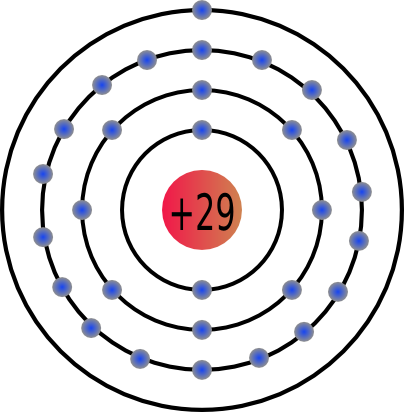
\includegraphics[width=0.25\textwidth]{./img/bohr-Cu}
\\
Kobberatom med 29 protoner og 29 elektroner.\\
Skall 1: 2 elektroner \\
Skall 2: 8 elektroner \\
Skall 3: 18 elektroner \\
Skall 4: 1 elektron
\\
Det ytterste elektronet har en svakere binding til kjernen.

TODO
